\documentclass[a4paper,12pt]{article}
\usepackage[T1]{fontenc}
\PassOptionsToPackage{defaults=hu-min}{magyar.ldf}
\usepackage[magyar]{babel}
\usepackage[a4paper]{geometry}
\geometry{margin=2cm}
\usepackage{graphicx}
\usepackage{fancyhdr}



\pagestyle{fancy}
\fancyhf{}
\fancyhead[LE,RO]{\normalfont\normalsize\thepage}
\fancyhead[RE]{\nouppercase{\sffamily\small\leftmark}}
\fancyhead[LO]{\nouppercase{\sffamily\small\rightmark}}


\begin{document}
\title{\textsc{Webprogramozás III. Gy. \\ {\normalsize (LBT\_IM744G2)}} \\ {\normalsize Beadandó feladat dokumentáció}}
\author{Kovács Norbert \\ ANOXWJ}
\maketitle
\newpage
\tableofcontents
\newpage


\section{Weboldal koncepciója}
\subsection{Technikai részletek}
A beadandó feladatot, az órán is alkalmazott \textit{xampp} szerverrel kívánom megvalósítani, \textit{apache netbeans} fejlesztőkörnyezettel. A Mysql kezelését a videóban is használt, \textit{phpmyadmin} oldalon intézem. Nem fontos részlet, a megvalósítás szempontjából, de a Windows operációs rendszer, virtuális gépként fut.

\begin{center}
	\textit{{\footnotesize (Követelmény: A beadandó feladat PHP MVC kereterendszerben készül!)}}
\end{center}

\begin{itemize}
	\item OS: Windows 10 Pro (21H1)
	\item Kernel: 10.0.19041.1023
	\item Mysql: 10.4.19-MariaDB
	\item PHP: 8.0.6
	\item Apache Netbeans IDE: 12.3
	\item CodeIgniter: 3.1.11
\end{itemize}

\subsection{Elképzelés}
A weboldal egy \textit{fiktív} szervezet köré épül, aminek a feladata  az \textit{állategészségügy}, és \textit{állatvédelem}. A fiktív szervezetnek több városban lesznek épületei országszerte. Egy városban több különféle épület is tartozhat a szervezethez. Például tartozhat állatmenhely, állatorvosi rendelő, raktárépület stb. Ezeknek az épületeknek vannak hozzájuk tartozó egységeik. Egy menhely állatok tárolására alkalmas kennelekkel, egy rendelő vizsgálóval, váróval, egy raktár szobákkal, szektorokkal rendelkezik stb.

Hasonlóképpen az egyetemi példafeladathoz, ahol
\begin{center}
	Kampusz -> Épület -> Terem \\[0.5cm]
	Pl.: Eger -> C épület -> 124-es terem,
\end{center}
felosztás található, itt is három rétegre kívánom felosztani a problémát, mégpedig:
\begin{center}
	Telep -> Épület -> 'Szoba'\\[0.5cm]
	Pl.: Miskolc -> Iroda -> 1-es iroda\\
	vagy\\
	Eger -> Egri állatmenhely -> 3-as Kennel.
\end{center}

A weboldal célja, tehát hogy a szervezet irányítani tudja a különböző városaiban található épületcsoportokat, pénzmozgásokat, alkalmazottakat stb.
A fiktív szervezetet, az előző beadandóm állatotthonából fejlesztem tovább, részben idő spórolás céljából, részben a hasonló koncepcióból adódóan.
 Szervezet neve: \textbf{Kék mancs}.

Az \textit{elképzelés} szerint, a felhasználókat több rétegben kezeljük majd. A weboldal nem a nyilvánosság felé közvetített oldal, hanem belső rendszerért felelős. Ettől függetlenül szükség lesz, telepenként admin, és felhasználói felületre. 


\section{Adatbázis tervezése}

Az első entitásunk, egy \textbf{Telep} entitás lesz. Itt nem egy konkrét Telephelyről van szó, hanem egy olyan összefoglaló jelzőről, mint az egyetem kapcsán a Campus-ról. Ennél találóbb, vagy pontosabb megnevezést nem tudtam kitalálni, ami összefoglalja az egy városban található épületcsoportokat. Szükségünk lesz, egy \textbf{épület} entitásra és egy '\textbf{szoba}' entitásra. Ennek a megnevezése, nem teljesen fedi le a pontos szerepet, hiszen minden épületben ez mást reprezentál, azonban szükséges eltárolnunk, hogy melyik állat melyik kennelhez van rendelve, vagy hogy melyik alkalmazott melyik irodában dolgozik stb. Itt majd valamilyen módon, implementálnunk kellene, egy hibakezelést, arra való tekintettel, hogy ne lehessen egy állatot, egy irodaszobához rendelni, vagy egy alkalmazottat, egy kennelhez. Szükségünk lesz egy \textbf{állat} entitásra is, hogy eltároljuk a különféle állatokat, amik a szervezethez köthetőek. Tárolnunk kell az \textbf{alkalmazottakat} is, és az \textbf{örökbefogadók} személyeit. Ezenkívül egy \textbf{Jogviszony} táblában, eltároljuk a munkaköröket, és a hozzájuk tartozó fizetést.

Ebben a felállásban is 8 forgalmi adattábláról van szó, ami túllépi a követelményben megjelölt minimális mennyiséget. Ahhoz, hogy a weboldal megközelítse a valóságban ,,alkalmazható'' jelzőt, még rengeteg entitásra lenne szükségünk, azonban az egyszerűség kedvéért nem bővítjük tovább az adatbázist, el kell fogadnom, hogy a jövőben ez okozhat \textit{hiányos funkciókat}.


\subsection{ER modell}
A pluszba kapott egyedi azonosító mezőket, és az idegen kulcsokat nem tüntetjük fel a tervezés során.

\begin{enumerate}
	\item Telep \\
	Egy Telep eltárolásához, elegendő a telep \textit{megnevezése} (ami gyakorlatilag a város neve), és egy \textit{leírás} mező.
	
	\item Épület \\
	Az épület entitás kapcsán, elég tárolnunk az épület \textit{megnevezését}, és \textit{típusát}.
	
	\item Szoba \\
	Egy épület alegysége, a szoba entitás lesz. Elegendő tárolnunk a \textit{típusát}, és a \textit{kapacitását}.
	
	\item Állat \\
	Egy állat esetén, tárolnunk kell a \textit{nevét}, \textit{típusát}, \textit{születési évét} és \textit{nemét}. Az állat \textit{életkora}, származtatott tulajdonság lesz.
	
	\item Alkalmazott \\
	Az alkalmazottak esetén, tároljuk el az alkalmazott teljes \textit{nevét}, a weboldalon használható \textit{felhasználónevét} és \textit{jelszavát}.
	
	\item Jogviszony \\
	A Jogviszonynak tároljuk a \textit{megnevezését}, és a \textit{fizetés értékét}. Mivel, nem lehet, két ugyanolyan megnevezésű munkakör, külön fizetéssel, ezért nincs szükségünk, külön azonosítómezőre. 
	
	\item Örökbefogadó \\
	Egy örökbefogadó személy kapcsán, el kell tárolnunk az \textit{nevét}, \textit{lakhelyét}, jelenleg birtokolt \textit{háziállatok számát},  és hogy \textit{javasolt-e örökbefogadásra}.
	
	\item Esemény \\
	Egy eseményről eltároljuk a \textit{megnevezését}, \textit{időpontját}, és \textit{leírását}.
\end{enumerate}

\begin{center}
	\includegraphics[width = 17cm]{"draw_io/SQL_tervezés.png"} \\
	{\small Az ER modell}
\end{center}

\begin{center}
	\textit{{\small ,,A megvalósítandó projekthez tartozó adatmodell legalább 5 forgalmi adattáblát tartalmaz (a külső modulok által használt táblákon kívül). Az adatmodell legalább 3. normálformában van és modellben megtalálható az egy-több, valamint a több-több típusú kapcsolat is. A technikai okokból létrehozott táblák (kapcsolótáblák) nem tekintendőek forgalmi táblának.''}}
\end{center}
\newpage
\subsection{Relációs adatmodell}
Az elkészült modell alapján, a következő táblák jöttek létre.
\begin{center}
	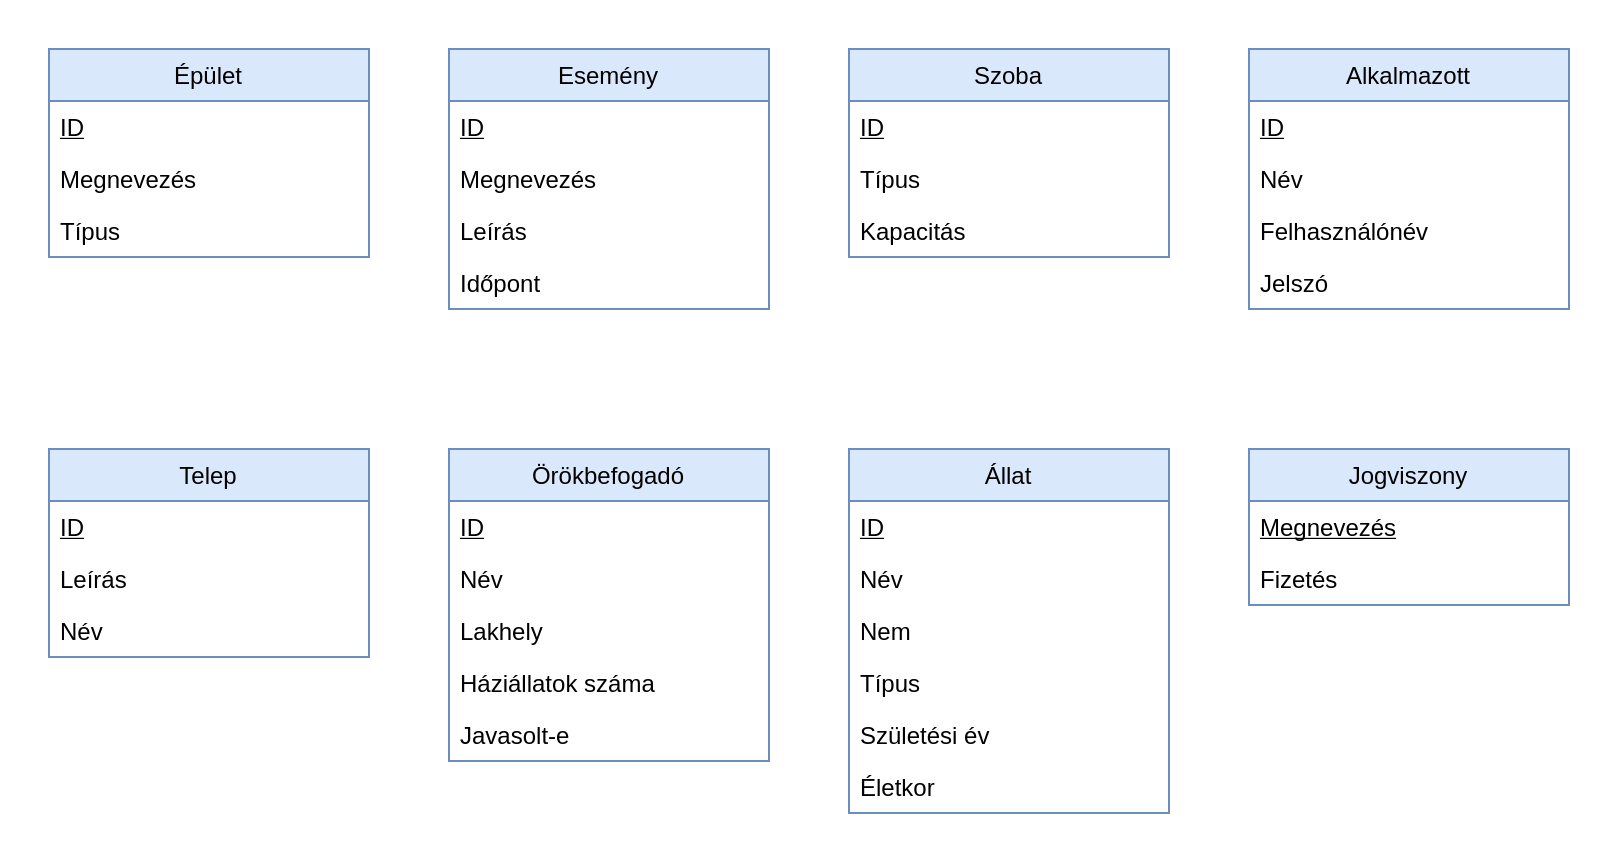
\includegraphics[width = 15cm]{"draw_io/SQL_Táblák.png"} \\
	{\small Az ER modell}
\end{center}
Hozzuk létre a szükséges kapcsolótáblákat, és illesszük be az idegen kulcsokat, majd jelöljük a kapcsolatokat.

\begin{center}
	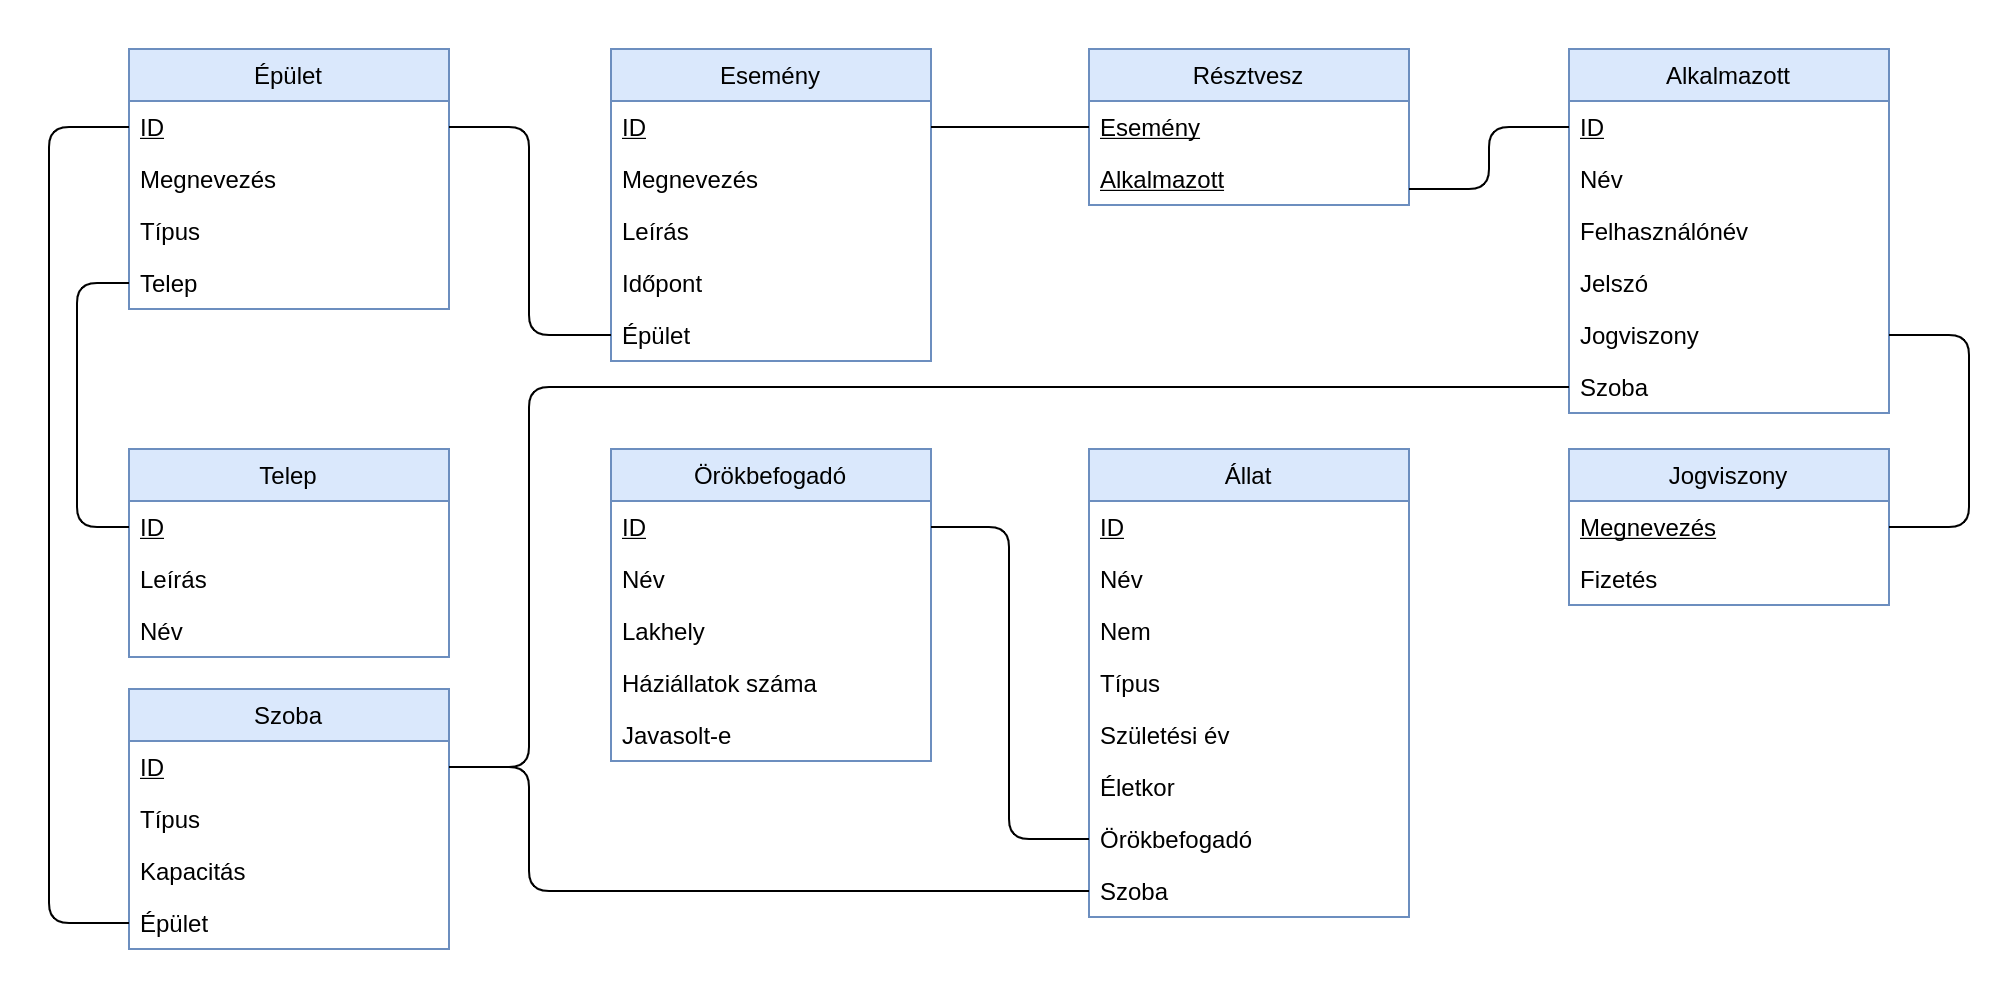
\includegraphics[width = 18cm]{"draw_io/SQL_Táblák_kapcsolatok.png"} \\
	{\small Az ER modell a kapcsolatokkal}
\end{center}
\subsection{SQL parancsok}
Az SQL parancsok megtalálhatóak az application/create.sql fájlban.
\section{Összefoglaló}


\end{document}
